\chapter{国内外研究现状}


\section{三维数字人角色外观生成}

\subsection{基于参数化模型的个性化外观生成}
基于参数化模型的个性化外观生成（personalized avatar appearance generation），通常以“可解释参数 + 可动画拓扑”作为结构先验：先用低维参数稳定刻画人体的形状、姿态和表情，再叠加衣物、头发、皮肤细节与材质纹理，最终获得“像本人、能驱动、可编辑”的数字人外观。人体的核心底座是 SMPL~\cite{SMPL2015}，其由体型与姿态相关的线性空间、蒙皮与校正项组成，在拓扑覆盖大量体型与自然姿态，便于跨帧对齐与工业管线接入。为了达到覆盖全身的效果，SMPL-X~\cite{SMPL-X:2019}将身体、手与脸整合到统一可微模型中，使得它们可以在同一参数空间里优化或回归，成为全身个性化建模与驱动的重要基础。头脸侧则以 FLAME~\cite{FLAME:SiggraphAsia2017}为代表，强调带关节结构（下颌、眼球等）与表情空间的解耦，支持表情编辑与动画适配。

\begin{figure}[h]
  \centering
  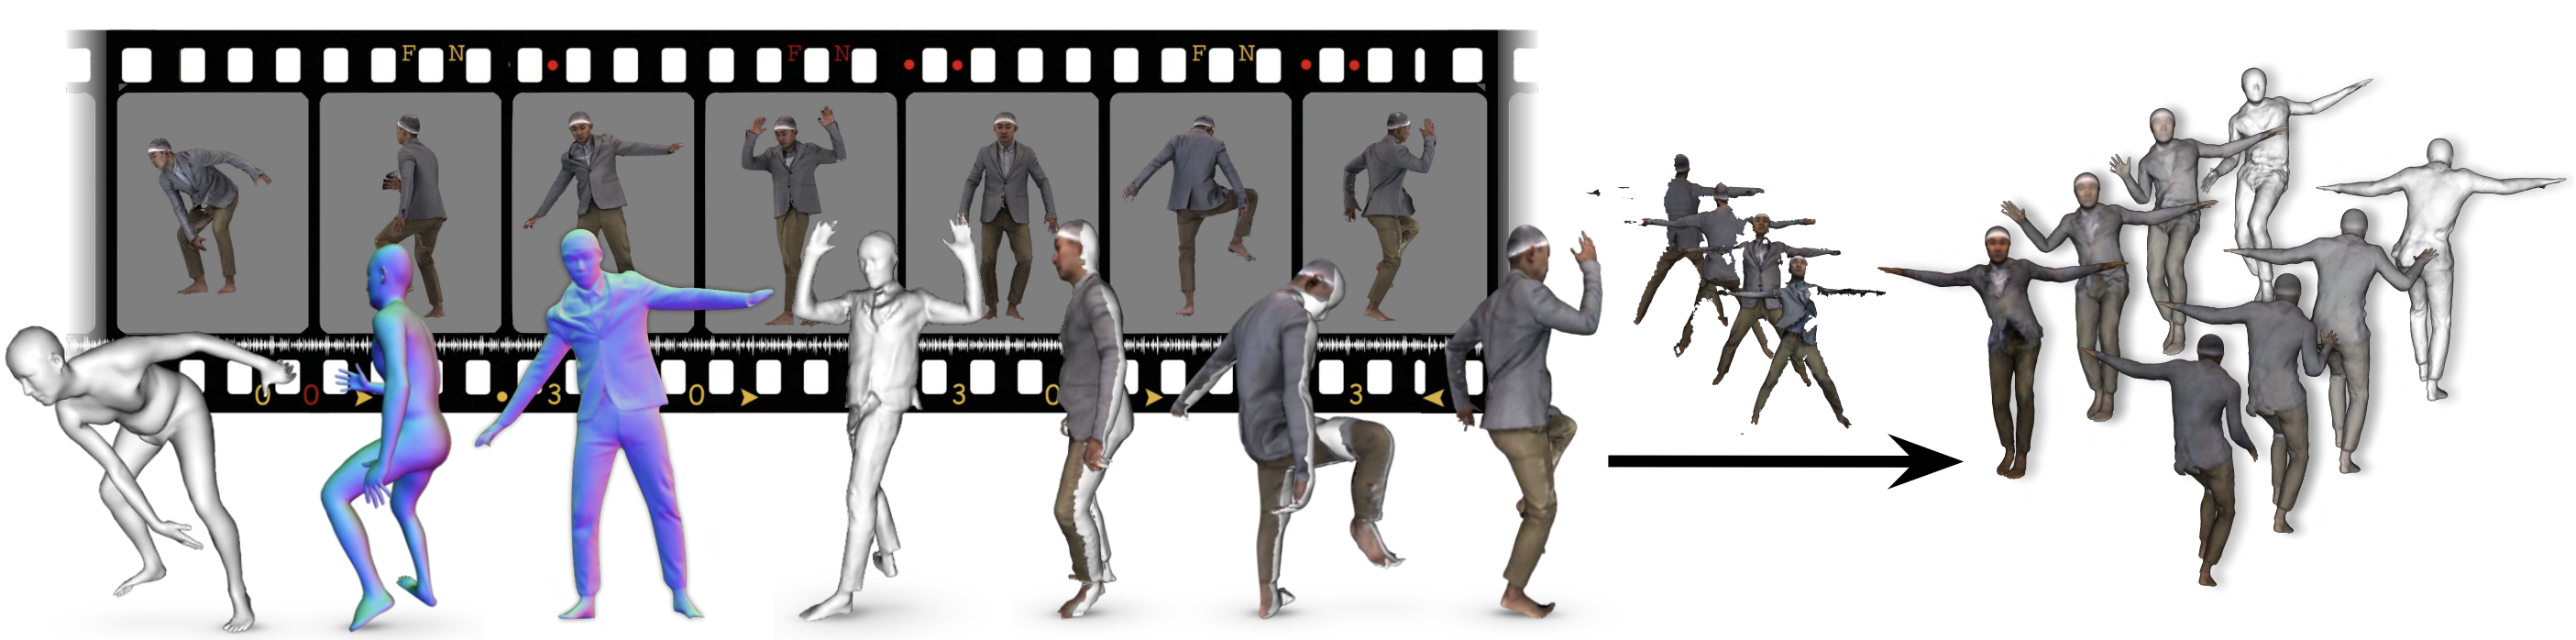
\includegraphics[width=1.0\linewidth]{figures/ICON.png}
  \caption{ICON实现的效果示意图（图片源自论文~\cite{xiu2022icon}）}
  \label{fig:ICON}
\end{figure}

然而，仅有“裸身参数化模型”难以表达衣物褶皱、发丝与局部材质，因此大量工作采用“参数化骨架/体表作为对齐引擎 + 高保真外观表示”的组合。ICON~\cite{xiu2022icon}是代表之一，如图~\ref{fig:ICON}所示，它以 SMPL/SMPL-X 提供姿态与体型先验，从自然图像估计法线并重建穿衣人体隐式表面，最后融合多帧得到可动画的个性化化身，显著增强了对 in-the-wild 姿态与遮挡的鲁棒性。面部方向，DECA~\cite{DECA:Siggraph2021} 在 FLAME 框架上学习与表情相关的细节（如皱纹随表情变化），提升单图重建的可动画真实感。神经渲染则更注重把外观细节强表示出来，NeuralBody~\cite{peng2021neural} 在 SMPL 引导下为动态人体学习隐式表示并整合多帧观测，改善稀疏视角下的新视角合成。随着 3D Gaussian Splatting~\cite{kerbl20233d} 兴起，GaussianAvatar~\cite{hu2024gaussianavatar}、3DGS-Avatar~\cite{qian20243dgs}等用显式高斯承载高频外观，在训练与渲染效率上更具优势，同时借助姿态驱动实现可动画 avatar。

\subsection{基于模型微调的个性化外观生成}
基于模型微调（fine-tuning）的个性化外观生成，指在一个预训练生成模型（常见为扩散模型、GAN，或用于3D表征上（如NeRF~\cite{mildenhall20nerf}或3DGS~\cite{kerbl3Dgaussians}），用少量目标样本对模型参数进行再训练，使模型能稳定生成同一角色的外观，并在不同提示词或条件下实现风格变化。其核心目标是同时满足三点身份一致、条件可控、多样性。

在2D图像个性化生成中，微调通常围绕扩散模型的去噪网络或其注意力模块展开，与只学习一个新token或embedding的轻量做法相比，微调能更充分地吸收目标主体的高频细节，例如发丝、细小配饰等。DreamBooth~\cite{ruiz2023dreambooth} 是 Ruiz 等人在提出的一类主体驱动（subject-driven）个性化方法，即给定某个具体主体的少量参考图片，对预训练的文本到图像扩散模型进行微调，使模型学会把一个稀有/唯一标识符 token（如 “[V]”）与该主体外观绑定。DreamBooth 的优势在于，样本需求低、身份还原强、并能与文本提示的场景结合得很好，因而在IP 形象生成和编辑等任务中非常实用。但它也有典型局限，微调可能把拍摄背景也学进身份，从而在大幅改变视角或遮挡时出现身份漂移。同时全量微调成本较高，权重管理不便，因此后来大量工作转向更轻量的参数高效微调（如 LoRA~\cite{hu2022lora}）或与 Textual Inversion~\cite{gal2022image} 等方法组合，以在质量与训练成本之间取得更好的折中。

\begin{figure}[h]
  \centering
  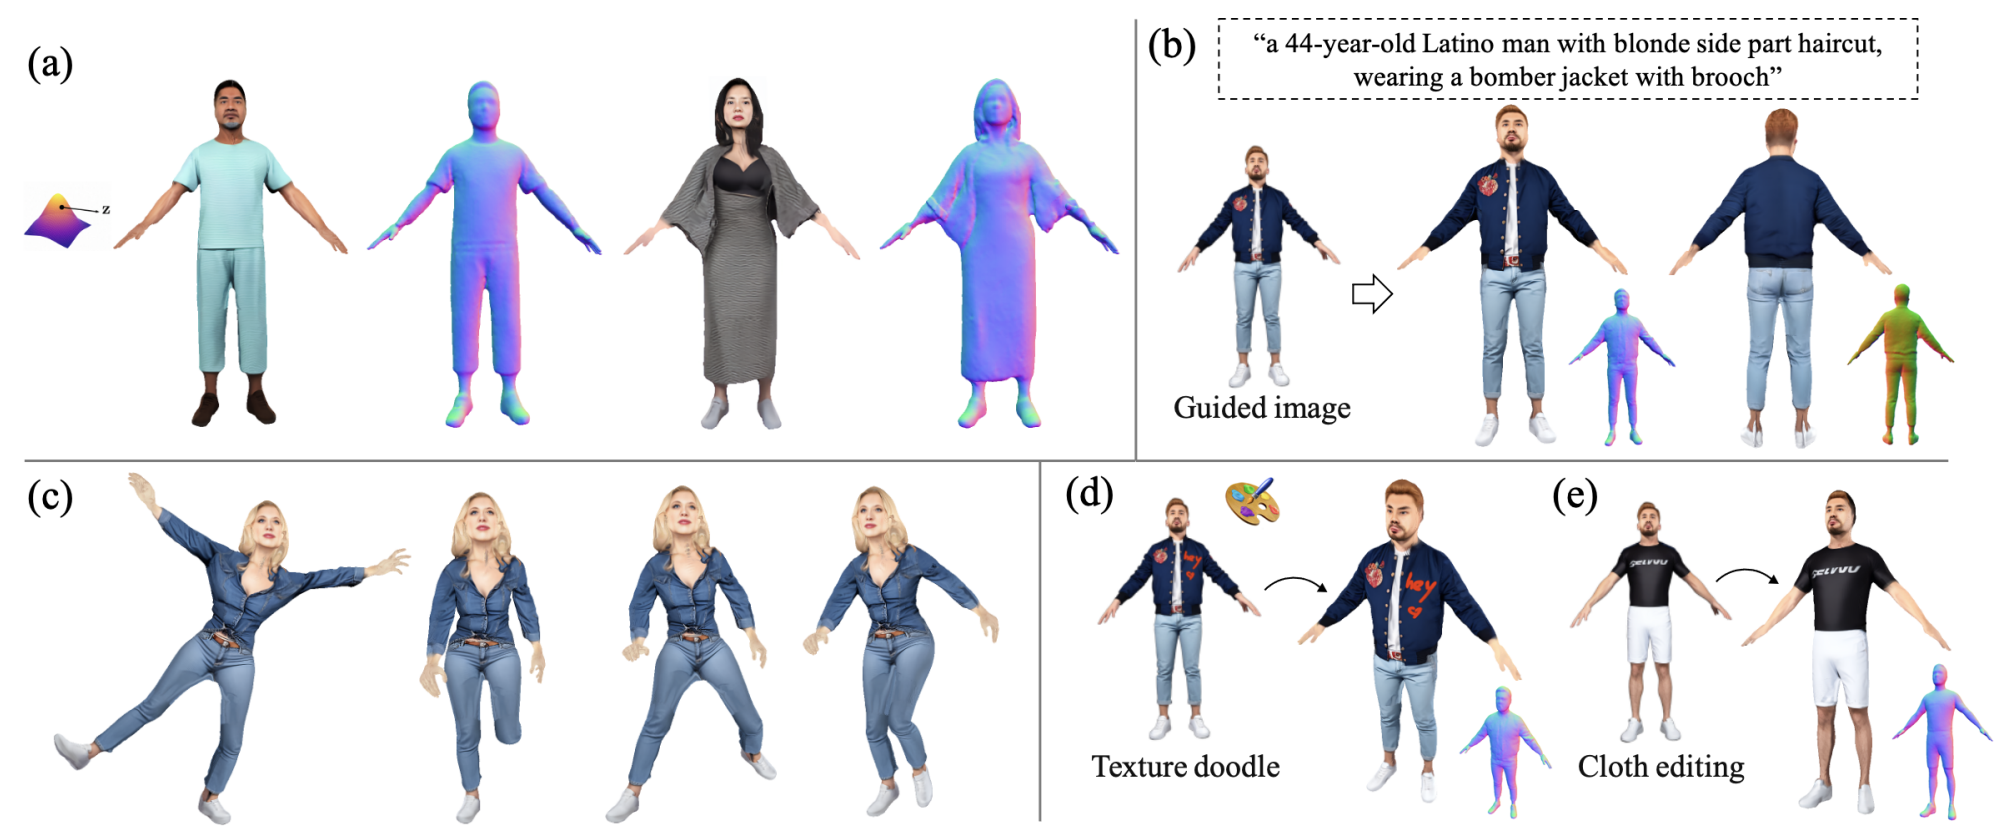
\includegraphics[width=1.0\linewidth]{figures/En3D.png}
  \caption{En3D算法流程示意图（图片源自论文~\cite{men2024en3d}）}
  \label{fig:en3d}
\end{figure}

在3D角色个性化生成中，微调是为某个主体训练专属的外观表示，例如为该人物拟合可新视角渲染的场景表示，并进一步通过骨架或形变场实现可驱动。En3D~\cite{men2024en3d}利用显式相机与SMPL结构化的多视角姿态条件，并通过扩散模型生成视角分布更均衡、内容更丰富的角色2D图像；随后基于 triplane 3D 生成器学习可泛化的 3D 表示。如图~\ref{fig:en3d}所示，在推理阶段，为弥补仅依赖 2D 监督信号可能带来的几何不精确，进一步引入多视角法线的几何雕刻优化以快速细化人体表面外观特征；同时结合语义 UV 分割与可微光栅化解耦显式纹理贴图，最终得到兼具真实外观、可编辑性与可动画驱动能力的高质量 3D 人体角色外观资产。

% 与只学习一个新token或embedding的轻量做法相比，微调能更充分地吸收目标主体的高频细节，例如发丝、细小配饰等。因此相似度往往更高，但风险也更大，模型可能过拟合到训练图的角度，出现复读同一张图、或把背景也当作身份特征。为缓解这一问题，常见策略是引入先验保持用同类别的通用样本约束模型不偏离原分布或者在损失设计上同时加上重建相似约束。

 
% \begin{figure}[h]
%   \centering
%   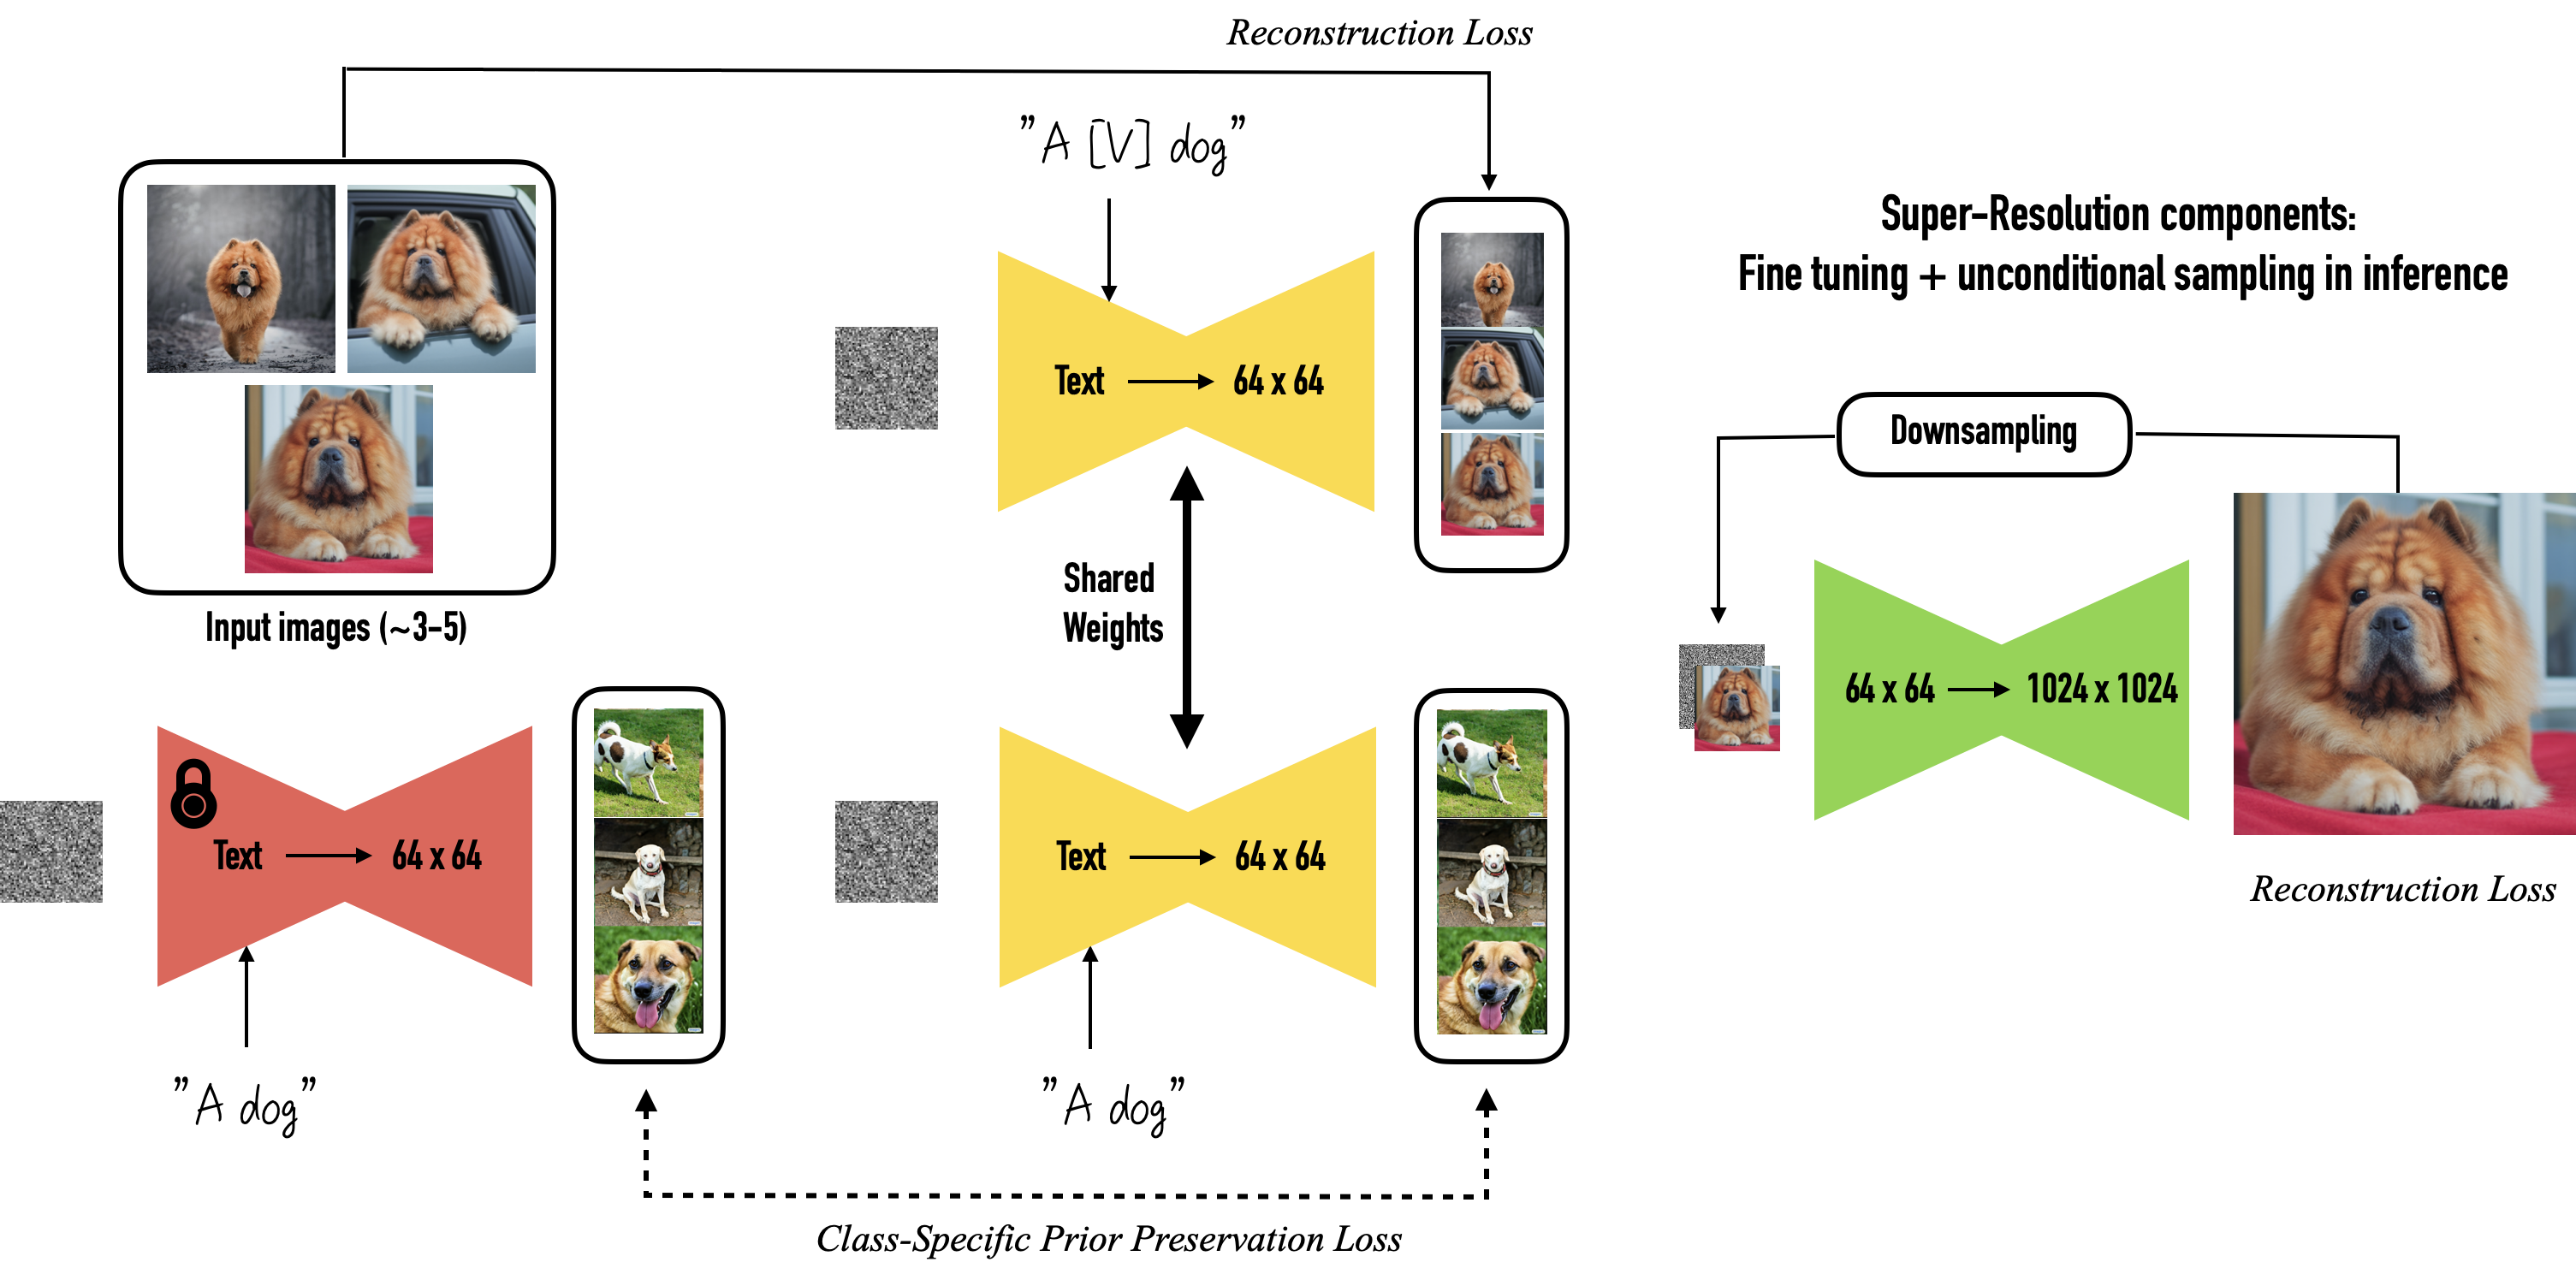
\includegraphics[width=1.0\linewidth]{figures/dreambooth.png}
%   \caption{DreamBooth框架示意图（图片源自论文~\cite{ruiz2023dreambooth}）}
%   \label{fig:dreambooth}
% \end{figure}

% DreamBooth~\cite{ruiz2023dreambooth} 是 Ruiz 等人在提出的一类主体驱动（subject-driven）个性化方法，即给定某个具体主体的少量参考图片，对预训练的文本到图像扩散模型进行微调，使模型学会把一个稀有/唯一标识符 token（如 “[V]”）与该主体外观绑定。之后用户只要在提示词里写“a photo of [V] person …”，模型就能在保持主体关键身份特征的同时，生成不同场景甚至艺术风格下的新图像，实现“把同一个人/物放到任意语境里”的再语境化生成。如图~\ref{fig:dreambooth}所示，它的核心训练机制是首先用主体参考图片和类别词（class name）的提示进行训练，例如“a [V] dog”，其中类别词让模型利用原本学到的“dog”语义先验，而“[V]”则承载主体参考图片中特定的身份信息。其次是DreamBooth 利用类先验保持损失（class-specific prior preservation loss），在微调时同时加入同类别的类图像和类提示词，鼓励模型在“dog”这一大类上仍保持原有多样性，避免少样本微调导致的过拟合、语言漂移或“复读训练图”。论文将其描述为一种自生成（autogenous）的先验保持机制，用模型自身对该类别的先验来约束更新幅度。


\subsection{基于注意力机制的个性化外观生成}

在扩散式文本生成模型中，个性化外观生成和编辑的关键难点是只改动用户指定的语义（如发色、服装等），同时最大化保留原主体的结构和纹理信息。注意力机制为这目标提供了天然的可控接口，其中交叉注意力（cross-attention）负责把文本对齐到空间区域与布局，自注意力（self-attention）则在生成过程中传播局部纹理与外观一致性。从而，许多研究围绕注意力的操控逐渐形成了一条无需或少量训练，以推理期控制为主的个性化外观编辑路线。

\begin{figure}[h]
  \centering
  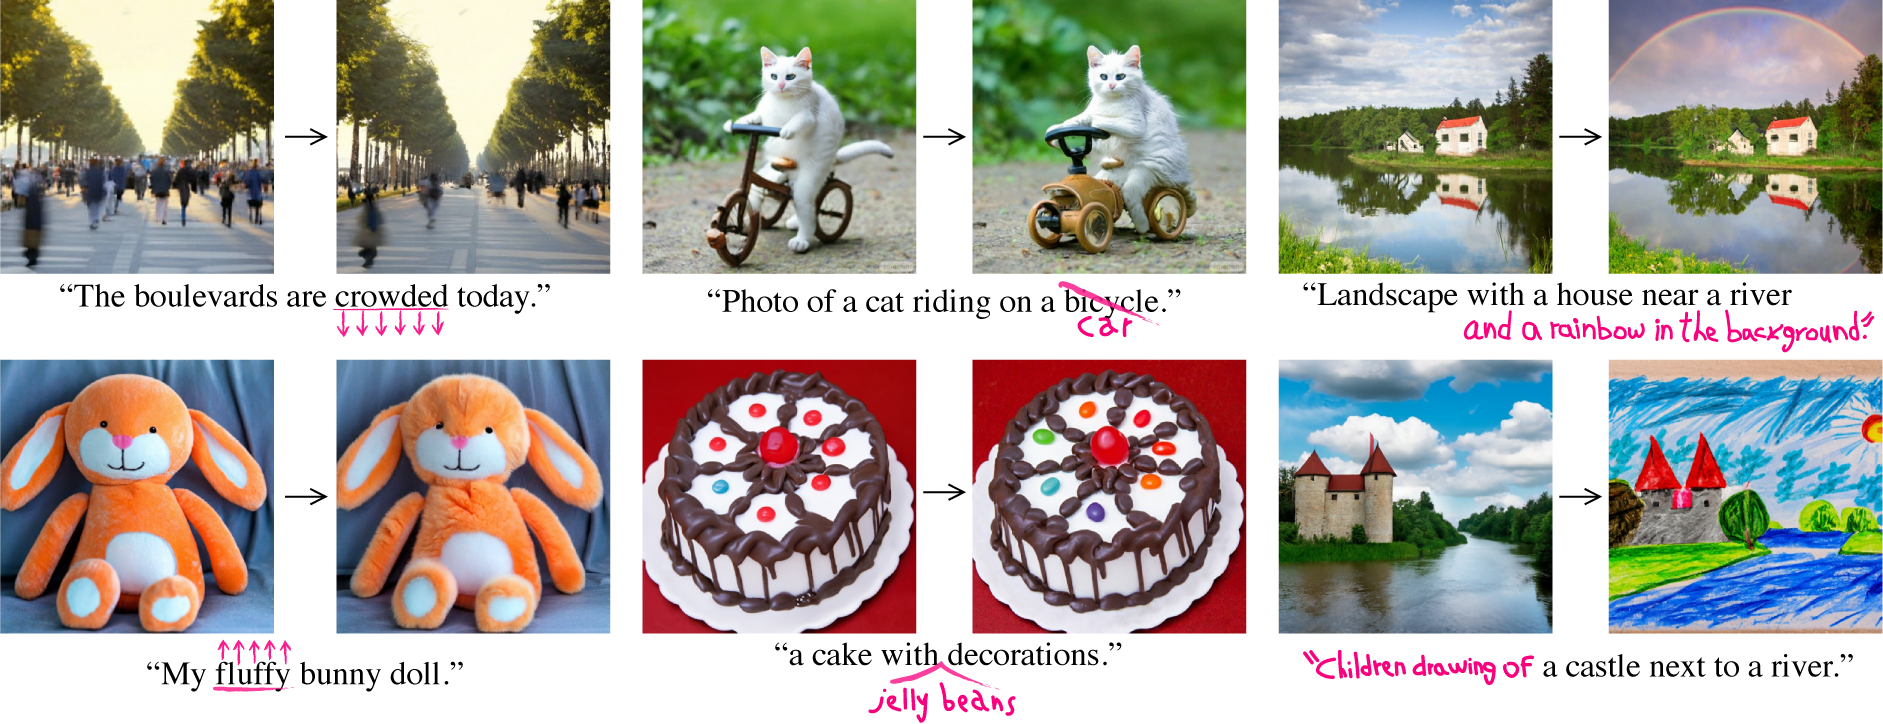
\includegraphics[width=1.0\linewidth]{figures/p2p.png}
  \caption{Prompt2Prompt图片编辑效果示意图（图片源自论文~\cite{hertz2022prompt}）}
  \label{fig:p2p}
\end{figure}

其中最具代表性的工作是Prompt2Prompt~\cite{hertz2022prompt}。Hertz等人发现在文本条件扩散模型里，交叉注意力层决定了每个词在图像的哪个区域起作用，而当我们只轻微修改提示词时，模型往往会因为注意力布局改变而生成完全不同的图。Prompt2Prompt 的核心思想是在编辑提示词生成时，把原提示词生成过程中的跨注意力图注入/对齐到新提示词的生成过程中，从而在结构层面锁定主体位置与构图，只让与被替换词相关的区域发生变化，实现文本驱动的局部编辑与身份保持，实现效果如图~\ref{fig:p2p}所示。具体而言，它提供了几种典型操作：（1）替换：用新词替换旧词，并把旧词对应的注意力分配到新词上，使同一位置出现新概念，如把“猫”替换为“狗”，但保留姿态与背景；（2）修饰：在不破坏原布局的前提下添加修饰语，如“红色”“金属质感”，让改动程度更渐进；（3）赋权：对特定词的注意力强度做权重调节，实现更像或更弱的可控变化。 另外，Prompt2Prompt 还用跨注意力图自动构造软掩码，在无需手工mask的情况下把编辑限定在目标区域，这对个性化外观尤其重要：既能避免背景被误改，也能减少主体身份特征漂移。
在真实图像个性化编辑中，Prompt2Prompt 往往与反演（inversion）配合：先把真实图映射回扩散的噪声轨迹，再在相同噪声起点上施加注意力控制完成编辑。Null-text Inversion~\cite{mokady2023null}是常用搭配，它在保留条件文本不变的前提下，仅优化 classifier-free guidance~\cite{ho2022classifier} 中的空文本嵌入，以获得更高保真的对应反演，使后续的 Prompt2Prompt 类编辑更稳定、更贴近原图身份与纹理。

除 Prompt2Prompt 外，注意力控制也被用于更复杂的外观一致性图片编辑。MasaCtrl~\cite{cao2023masactrl}将扩散模型的自注意力改造为“互注意力（mutual self-attention）”，在编辑时从源图的相关区域查询纹理与局部细节，从而在非刚性变化下更好地保持外观一致，并可用跨注意力自动得到的掩码引导前景和背景解耦。Attend-and-Excite~\cite{chefer2023attend} 则从另一个角度利用注意力，当模型出现忽略某些词或属性绑定错误时，它在推理期直接提升对应词的注意力响应，减少语义遗漏与错绑，提高文本语义与生成结果的一致性，这对描述驱动的个性化外观生成同样有帮助。


\section{三维数字人舞蹈动作生成}
舞蹈动作生成的研究重点集中在如何精准建模舞蹈演员的细腻动作，构建高质量的数据集，以及如何有效生成表现力丰富且与音乐协调的三维舞蹈动作。然而，由于舞蹈动作本身的复杂性，包括身体运动、手势、表情等多种信息，以及动作与音乐节奏、情绪之间的精细交互~\cite{1016154760, MYSY202106014}，目前国内外学术界在舞蹈数据采集、动作编码和动作生成方法等方面仍面临诸多挑战。因此，深入探讨舞蹈动作生成技术的关键问题，特别是在数据集构建、动作表征学习和跨模态生成算法方面的最新研究进展，对于推动该领域的技术发展具有重要的理论与实践意义。

\subsection{三维动作编码}
向量量化（Vector Quantization, VQ）是一种核心的数据压缩技术，最初被提出用于减少数据存储空间与传输带宽需求，其本质是将连续的高维向量通过聚类或映射方式对应到一个预先设计好的离散码本（codebook）中的有限项，从而实现数据的高效压缩与重建~\cite{gray1998quantization}。近年来，随着深度学习的发展，VQ 技术被广泛地应用于生成式建模领域，特别是在向量量化变分自编码器（Vector Quantized Variational Autoencoder, VQ-VAE）中的应用~\cite{van2017neural}。VQ-VAE 在传统变分自编码器的基础上，通过引入离散的潜变量表示，克服了连续潜变量的平滑性问题，实现了更为清晰和高效的潜在空间表征。这一方法极大地启发了人体动作生成领域的相关研究，如 TM2T~\cite{guo2022tm2t} 与 Bailando~\cite{siyao2022bailando} 等模型，通过使用 VQ-VAE 对连续的人体动作进行离散化表示，以实现高效动作编码。

为进一步提升基于 VQ 方法对人体运动特征的表示能力，近期的一些研究提出了不同的优化策略与扩展方法。例如，T2M-GPT~\cite{zhang2023t2m} 提出了指数移动平均（Exponential Moving Average, EMA）与码本重置（code reset）机制，这些机制有效解决了传统 VQ 码本容易退化的问题，从而显著提升了基于 VQ 模型的动作表示质量。与此同时，HumanTomato~\cite{lu2023humantomato} 与 DanceMeld~\cite{gao2023dancemeld} 等研究引入了分层向量量化（Hierarchical Vector Quantization），通过构建多级的码本结构，捕捉不同粒度层次的动作特征，从而提升动作细节的重建能力。尽管上述方法取得了显著的进展，向量量化过程本身所固有的量化误差仍然是制约性能进一步提升的重要挑战之一。针对该问题，残差向量量化（Residual Vector Quantization, RVQ）技术应运而生~\cite{zeghidour2021soundstream, borsos2023audiolm}。RVQ 方法通过在多层级结构中逐步量化残差信息，以迭代方式优化编码结果，从而在每一步有效降低量化误差并提高动作表示的精确性。近期，MoMask~\cite{guo2024momask} 等研究已将 RVQ 应用于动作生成领域，并证实了其在减少重建误差与增强动作细节捕捉方面的显著优势。

然而，当前现有的基于 VQ 与 RVQ 的方法仍存在一定局限，尤其是在建模复杂的整体动作交互方面缺乏对动作部位之间层次关系的显式捕捉与表达能力。这种不足导致现有方法在面对舞蹈等复杂、高表现力动作生成任务时表现不足。因此，如何有效构建兼顾全局与局部特征层次化表达的量化方法，将成为该领域进一步研究的重要方向之一。

\subsection{三维舞蹈动作数据集}
现有的三维（3D）人体动作数据集已经相当丰富，规模和质量也在持续提升~\cite{Plappert2016, Guo_2022_CVPR, li2022danceformer, lin2023motionx, zhang2025motion, KM2D}。例如，最新发布的 Motion-X++~\cite{zhang2025motion} 数据集包含超过 12 万段 3D 全身动作序列及对应标注 。然而，与日常动作数据相比，舞蹈类 3D 动作数据在现实生活中出现频率较低，其采集往往需要专业舞者参与并借助复杂设备，这使得数据获取成本高、效率低，因而现有舞蹈动作数据集在数量和质量上仍存在不足。目前公开的舞蹈数据集主要通过三种途径构建，各有局限：其一，二维关键点序列表示的舞蹈数据~\cite{lee2019dancing2music, lee2018listendance, li2022danceformer}，这类数据仅包含二维平面的骨架关键点轨迹，缺乏真实的三维结构信息。其二，多视角视频重建的三维舞蹈数据~\cite{li2021ai, le2023music}，通过多视角同步摄像获取舞蹈视频并重建三维姿态，虽然捕捉了三维位姿数据，但通常精度不高（如图~\ref{fig:aistpp_data_pipline}所示为该类数据集的采集流程）。典型例子是AIST++ 舞蹈数据集，如图~\ref{fig:aistpp_data_pipline}所示，它利用多视角视频估计出共 1408 段 3D 舞蹈骨骼序列，涵盖 10 种舞蹈流派，每段动作 7.4 至 48 秒不等。第三，动作捕捉（MoCap）获取的舞蹈数据~\cite{valle2021transflower, tang2018dance, zhuang2022music2dance}，此类数据集通过光学动作捕捉直接记录舞者的 3D 动作轨迹，具有较高的准确度，但由于设备昂贵和采集耗时，总时长普遍较短，风格和演员多样性也有限。并且这类动捕舞蹈数据通常缺乏手部动作细节，舞蹈风格与舞者类型多样性不足。

\begin{figure}[h]
  \centering
  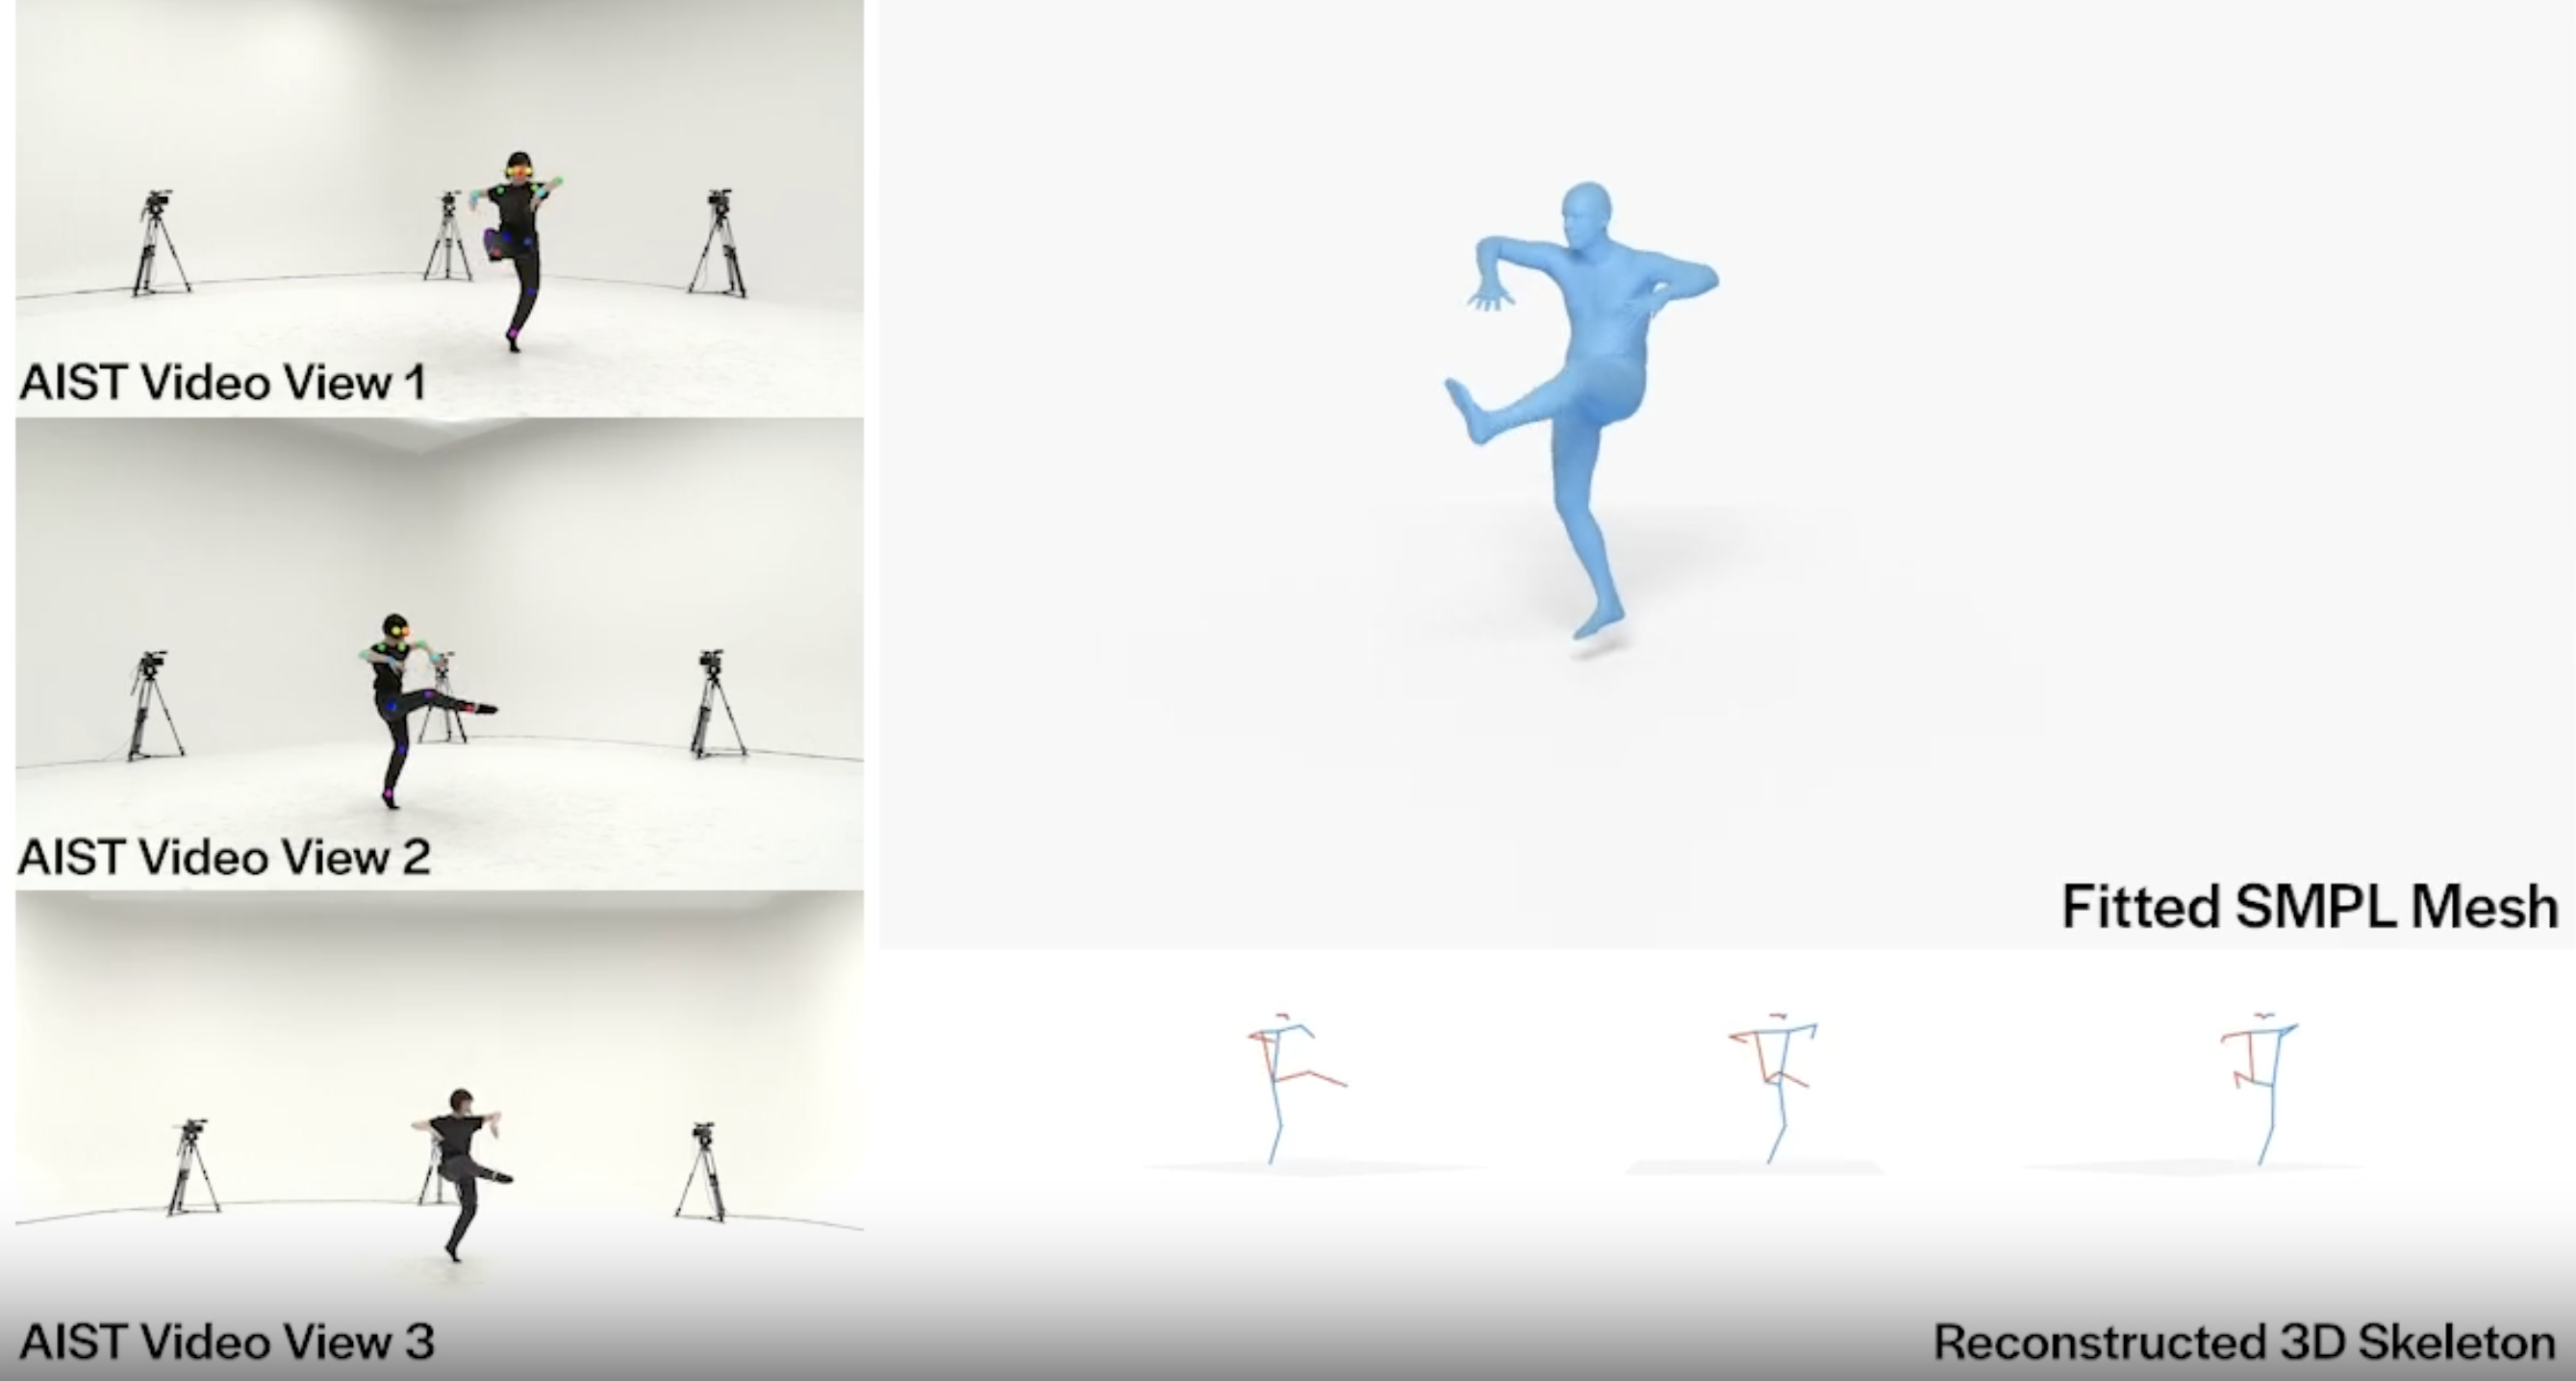
\includegraphics[width=0.8\linewidth]{figures/aistpp_data_pipline.png}
  \caption{AIST++舞蹈动作数据集采集方法~\cite{li2021ai}}
  \label{fig:aistpp_data_pipline}
\end{figure}

FineDance 数据集~\cite{li2021ai}的提出在一定程度上缓解了上述问题。FineDance 采用动作捕捉系统采集了 14.6 小时的舞蹈动作数据，涵盖 346 支舞曲，由专业舞者完成，能够提供精确的身体和手部运动细节。该数据集细分了 22 种舞蹈流派，在舞蹈种类多样性上显著优于以往数据集。不过，它并未采集面部表情信息，群舞场景的数据也未涉及，仍存在进一步提升空间。近年来国内外也涌现出一些新的大型多人舞蹈相关数据集。例如，AIOZ-GDANCE 数据集~\cite{le2023music}从网络视频中半自动提取了 16.7 小时配乐对齐的 3D 舞蹈动作，涵盖7种舞蹈风格和 16 类音乐类型。但是精度较低，可用性差。
尽管这些新数据集在规模和多模态方面有了长足进展，当前仍缺乏一个在数据规模、动作精度、细节完整性（涵盖面部、手部）和风格多样性上全面均衡的3D 舞蹈数据集，这也成为舞蹈动作研究领域亟待解决的核心问题之一。

\subsection{基于检索拼接的三维动作生成}
早期的音乐驱动舞蹈合成主要采用基于音乐线索的检索方法。从预先录制的舞蹈数据库中按照音乐节奏或风格检索出匹配的片段，再进行拼接生成整段舞蹈。例如，Arikan 等人和 Kim 等人早期的研究工作通过匹配音乐节拍与现有动作库中的舞蹈单元，实现了交互式或节奏同步的舞蹈生成~\cite{arikan2002interactive, kim2003rhythmic, shiratori2006dancing, kim2006making}。这类方法在一定程度上保证了舞蹈与音乐的同步性，但由于仅依赖低层次的音乐特征匹配，无法捕捉音乐与舞蹈动作之间复杂而内在的对应关系。因此，生成的舞蹈缺乏多样性和创造性，舞蹈表现力受到限制。

\subsection{基于扩散模型的三维动作生成}
近年来，扩散模型作为生成领域的新进展被引入音乐到舞蹈生成中，显著提高了动作生成的逼真度和多样性。扩散模型通过逐步添加和去除噪声来生成数据，具有建模复杂分布的强大能力，因而有助于生成更生动流畅的舞蹈序列。Tseng等人提出的EDGE~\cite{tseng2023edge}方法将扩散模型与音乐特征提取网络相结合如图~\cite{tseng2023edge}所示，能够生成与输入音乐高度契合且物理上合理的舞蹈动作。该方法还支持对生成过程的编辑控制，例如指定部分关节动作或插入过渡片段，实现了生成结果的可编辑性。此类基于扩散的模型在定量评估的物理合理性、节奏同步和动作多样性方面相比先前方法有了显著提升。一些研究也开始关注长序列舞蹈的生成：Li等人开发了Lodge~\cite{li2024lodge}系列模型，采用从粗到细的分层扩散生成策略，能够在保证局部动作稳定性的同时生成超长的舞蹈序列。尽管扩散模型展现了强大的生成能力，直接将音乐映射为高维三维关节序列仍面临挑战——如果缺乏适当约束，可能出现动作失真或偏离真实舞蹈分布的情况。因此，为确保生成动作符合人类舞蹈的运动学规律，最新的方法往往在扩散生成过程中融入物理约束或分层生成策略，以减轻上述不稳定性问题。总体而言，扩散模型推动了音乐驱动舞蹈生成质量的大幅提升，但如何平衡高自由度生成与动作的真实性分布仍需进一步研究。

\begin{figure}[h]
  \centering
  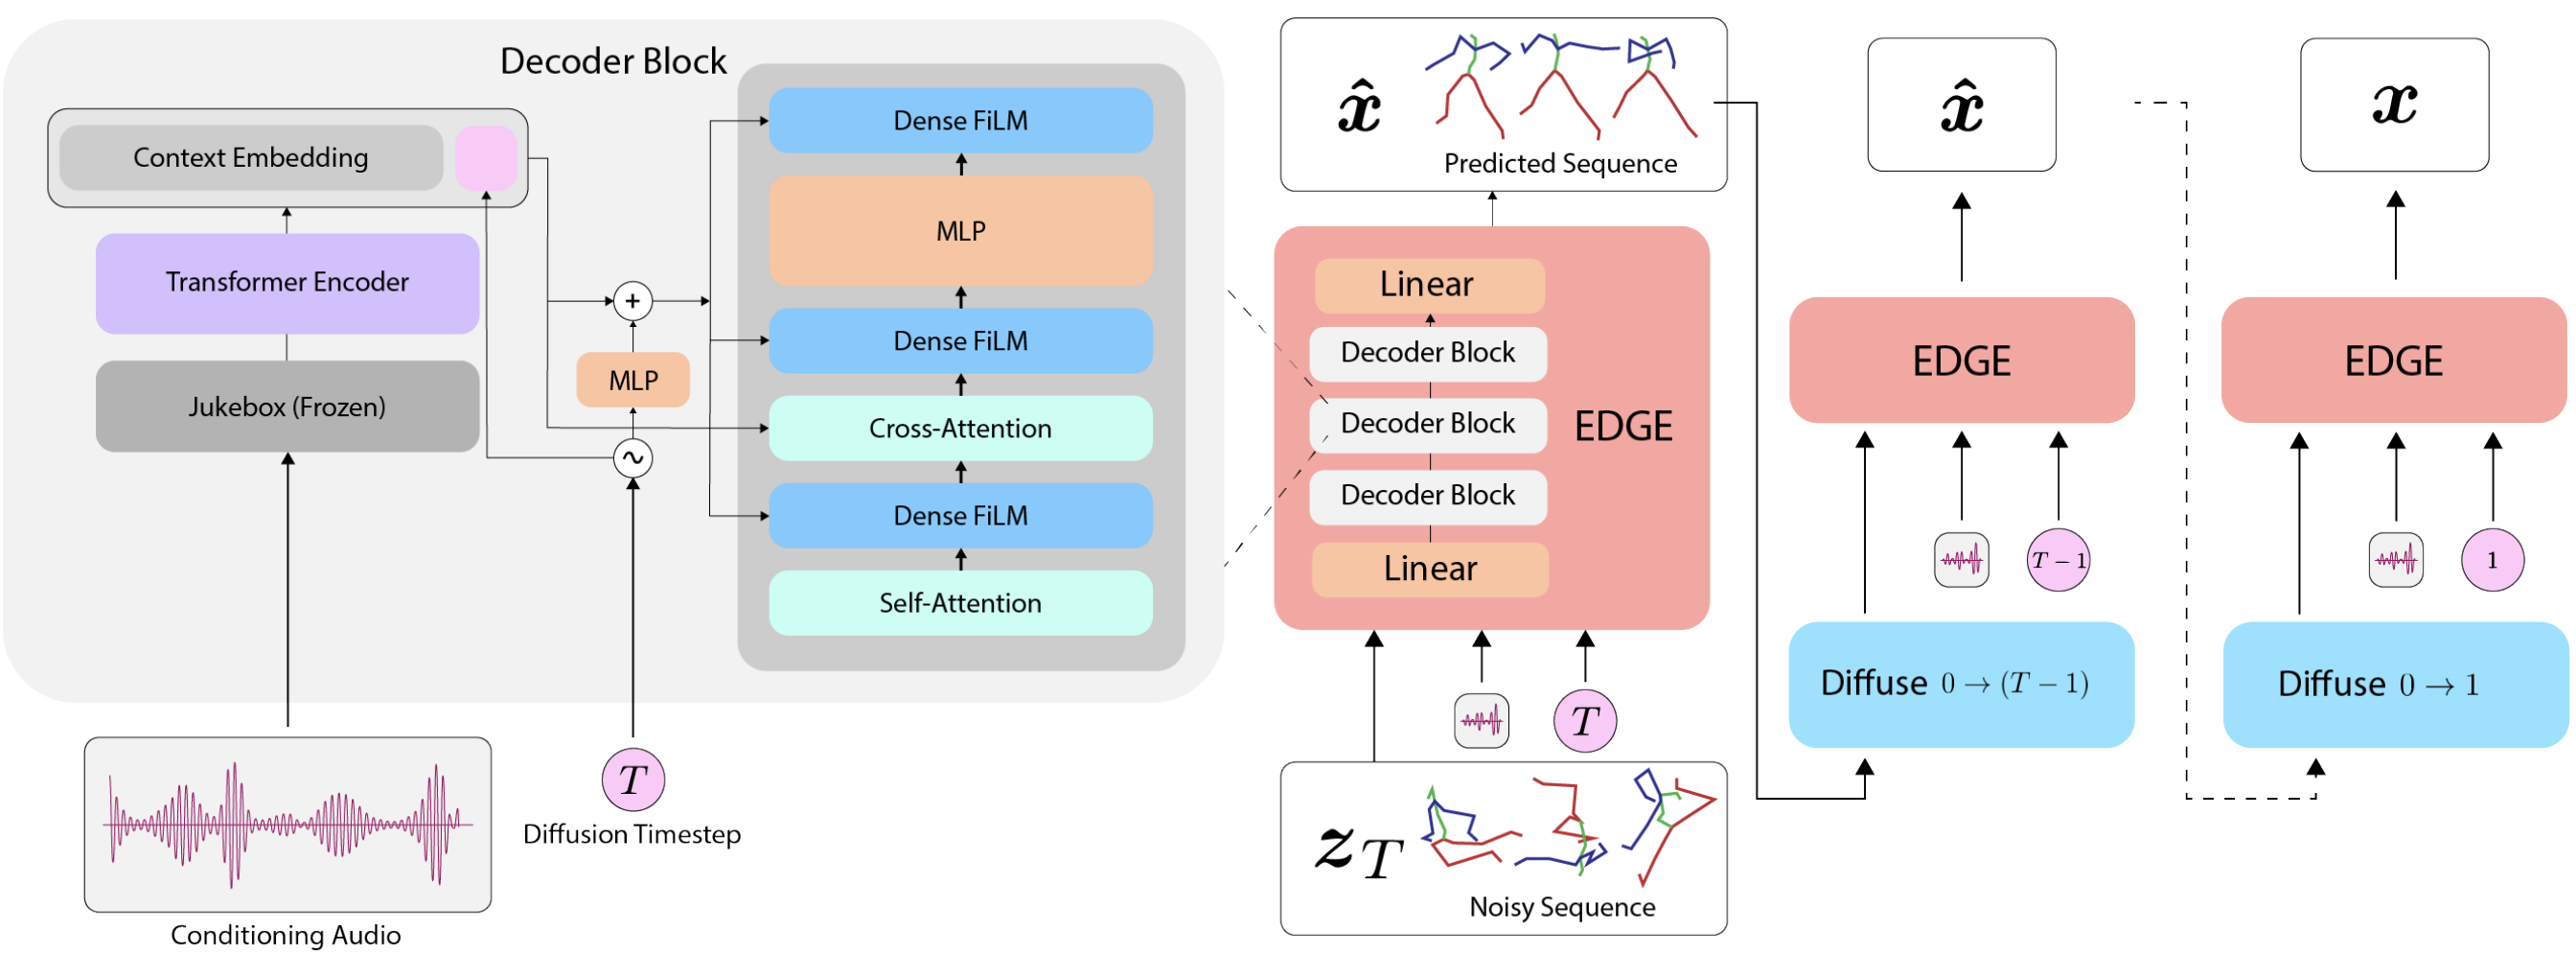
\includegraphics[width=1.0\linewidth]{figures/EDGE.png}
  \caption{EDGE舞蹈动作生成框架示意图（图片源自论文~\cite{tseng2023edge}）}
  \label{fig:edge}
\end{figure}

\subsection{基于自回归模型的三维动作生成}
随着深度学习的发展，研究者开始将音乐驱动的舞蹈合成视为生成任务，采用数据驱动模型直接学习音乐到动作的映射。Tang等人构建了包含多种舞蹈类型的音乐-舞蹈数据集，并使用长短期记忆网络（LSTM）自动编码器提取音乐与动作特征间的映射关系，实现了早期的深度生成舞蹈模型~\cite{tang2018dance}。Li等人提出了AI Choreographer模型，将 Transformer~\cite{vaswani2017attention} 引入舞蹈生成，提高了生成舞蹈的连贯性和平滑度~\cite{li2021ai}。同时，一系列基于生成对抗网络（GAN~\cite{goodfellow2020generative}）和更复杂Transformer架构的方法相继出现，在生成动作质量上取得了明显提升。例如，DanceFormer~\cite{li2022danceformer}采用两阶段的Transformer框架，先根据音乐生成关键肢体姿态，再进行插值补全细节，以保证动作序列的连贯与合理。又如Bailando~\cite{siyao2022bailando}框架引入了双阶段的生成方法，如图~\ref{fig:bailando}所示，首先是舞蹈记忆模块将舞蹈序列离散成语义单元，再通过Actor-Critic GPT生成器在强化学习的奖励引导下将这些单元编排成与音乐节奏协调的连续舞步。这些深度生成模型有效学到了音乐与动作之间的关联特征，生成结果相比早期检索方法更加平滑自然。然而，它们仍存在不足之处，比如生成的编舞往往欠缺真实舞蹈应有的动态变化和多样性，容易出现动作模式单一或重复的现象。

\begin{figure}[h]
  \centering
  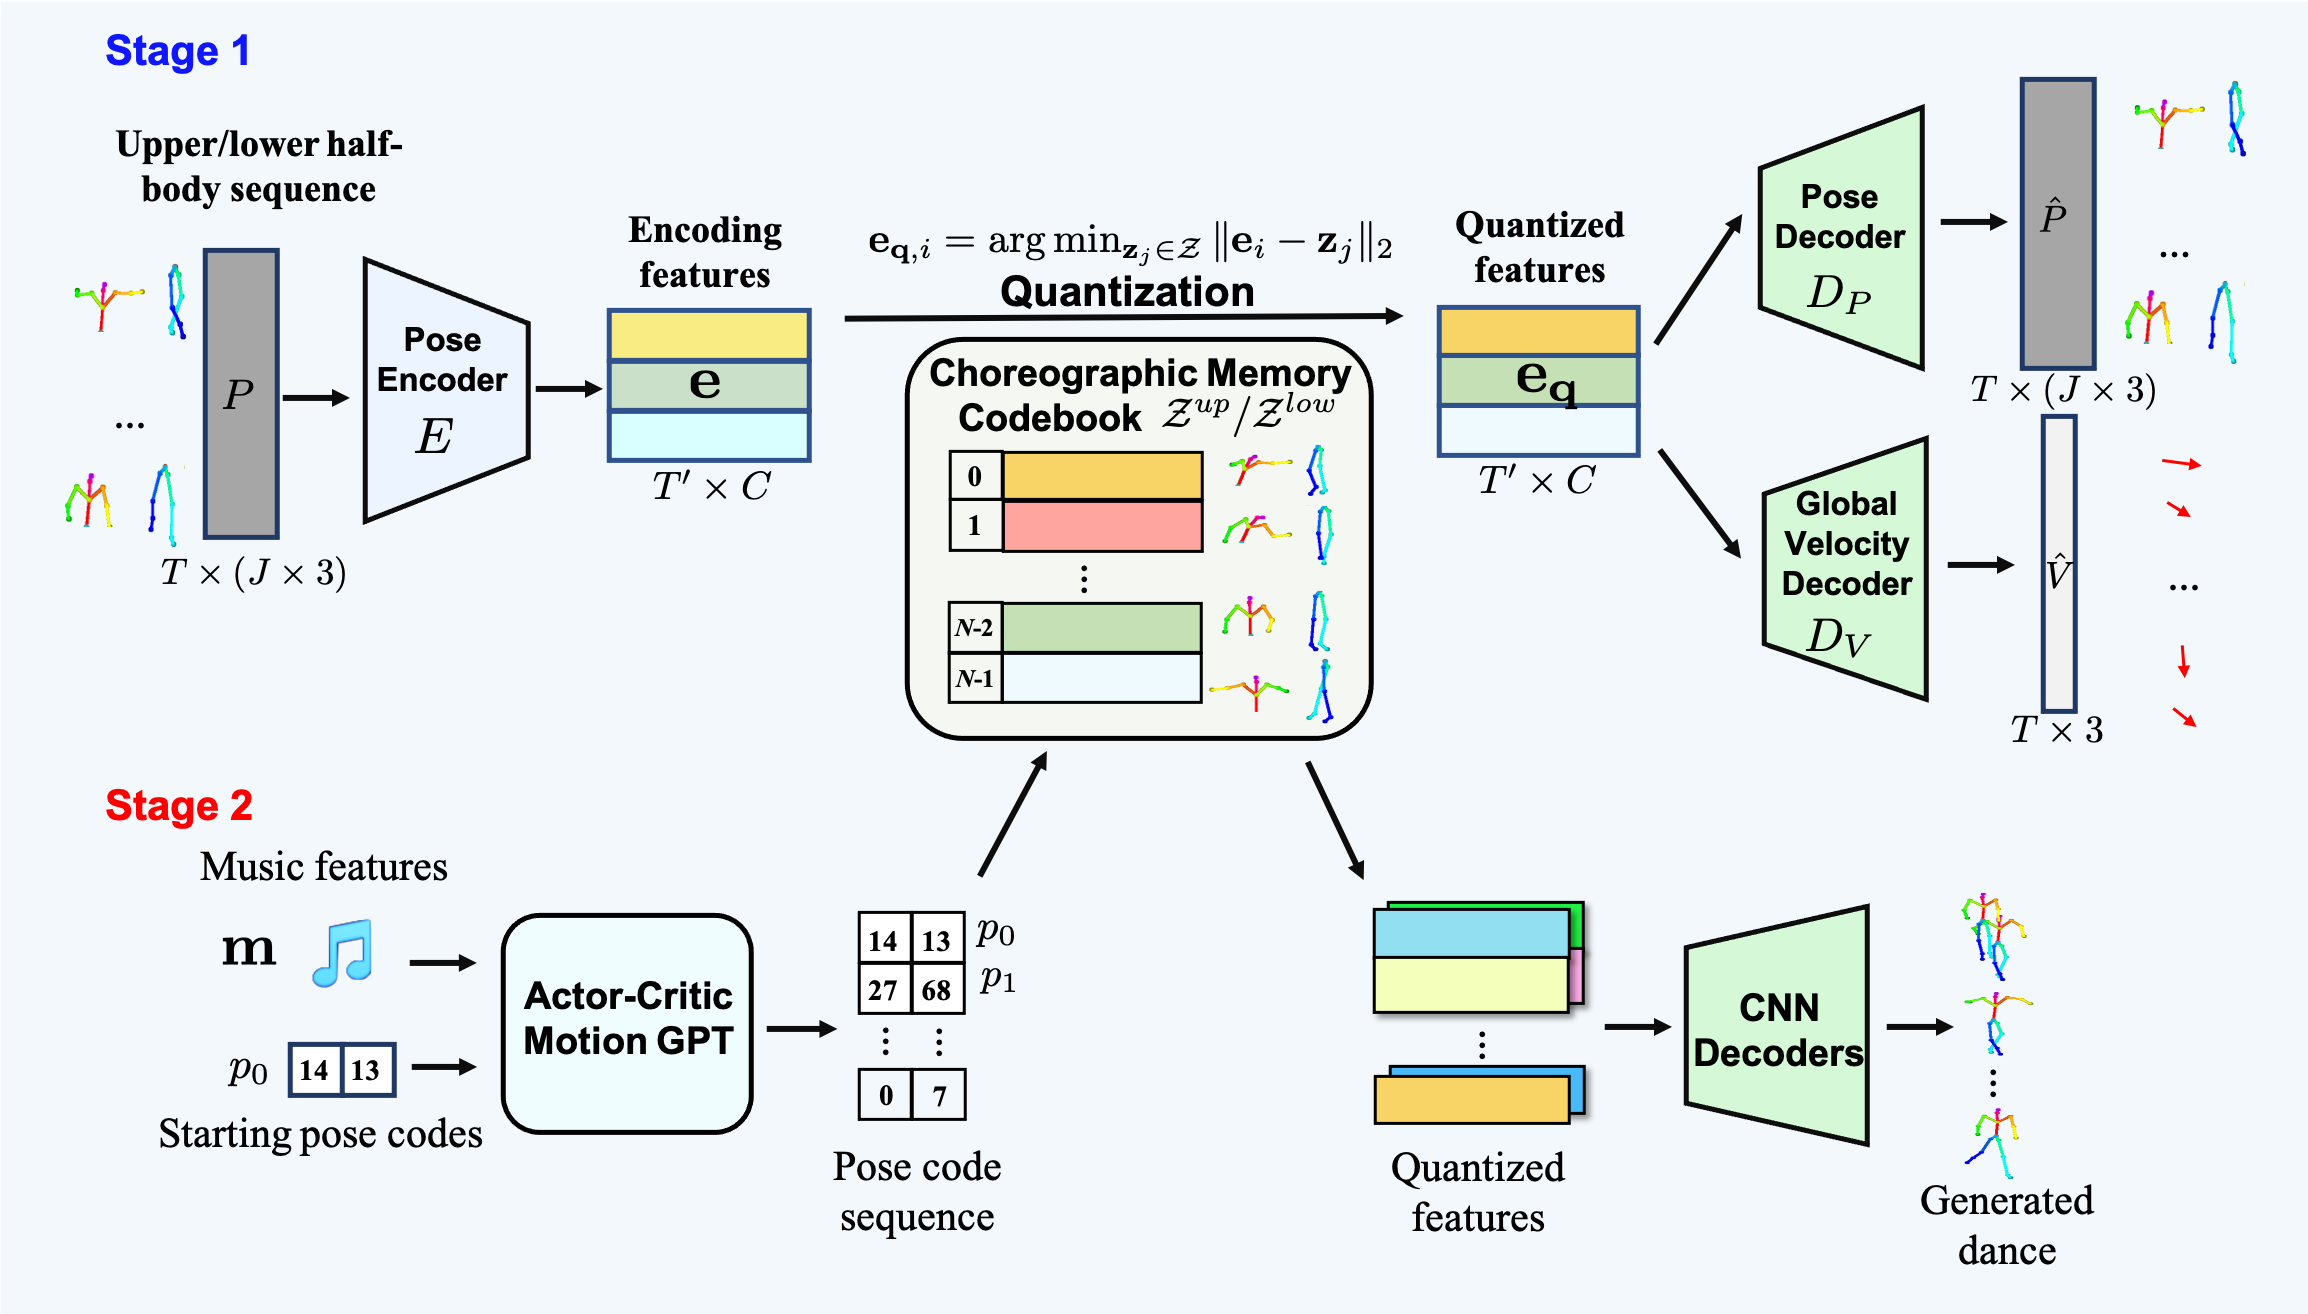
\includegraphics[width=1.0\linewidth]{figures/Bailando.png}
  \caption{Bailando舞蹈动作生成框架示意图（图片源自论文~\cite{siyao2022bailando}）}
  \label{fig:bailando}
\end{figure}

% 近年来，扩散模型作为生成领域的新进展被引入音乐到舞蹈生成中，显著提高了动作生成的逼真度和多样性。扩散模型通过逐步添加和去除噪声来生成数据，具有建模复杂分布的强大能力，因而有助于生成更生动流畅的舞蹈序列。Tseng等人提出的EDGE~\cite{tseng2023edge}方法将扩散模型与预训练的音乐特征提取网络相结合，能够生成与输入音乐高度契合且物理上合理的舞蹈动作。该方法还支持对生成过程的编辑控制，例如指定部分关节动作或插入过渡片段，实现了生成结果的可编辑性。此类基于扩散的模型在定量评估的物理合理性、节奏同步和动作多样性方面相比先前方法有了显著提升。一些研究也开始关注长序列舞蹈的生成：Li等人开发了Lodge~\cite{li2024lodge}系列模型，采用从粗到细的分层扩散生成策略，能够在保证局部动作稳定性的同时生成超长的舞蹈序列。尽管扩散模型展现了强大的生成能力，直接将音乐映射为高维三维关节序列仍面临挑战——如果缺乏适当约束，可能出现动作失真或偏离真实舞蹈分布的情况。因此，为确保生成动作符合人类舞蹈的运动学规律，最新的方法往往在扩散生成过程中融入物理约束或分层生成策略，以减轻上述不稳定性问题。总体而言，扩散模型推动了音乐驱动舞蹈生成质量的大幅提升，但如何平衡高自由度生成与动作的真实性分布仍需进一步研究。
  
为了进一步提高音乐驱动舞蹈生成的表现力和精准性，近年来的研究开始融合多模态信息并利用大规模预训练模型的知识来改进生成过程。一方面，音乐本身包含丰富的情感和语义信息，传统方法使用的手工特征（如MFCC、节拍等）难以充分表征这种关联。为此，研究者引入了预训练的音乐基础模型来提取高层语义特征。例如，Tseng等人 EDGE~\cite{tseng2023edge} 中利用OpenAI的Jukebox~\cite{dhariwal2020jukebox} 模型提取音乐嵌入，从而获取比简单频谱特征更具表现力的音乐语义信息。又有研究将 Wav2CLIP~\cite{wu2022wav2clip} 这类跨模态音频模型提取的深层特征与传统音频特征结合，使生成的舞蹈序列在风格和细节上与音乐更加契合。另一方面，除了音乐信号之外，融合其他模态的信息也成为趋势。例如，通过文本提示指定舞蹈风格或情绪，利用大模型（如CLIP~\cite{radford2021learning}）将文本与舞蹈动作空间联系起来，从而实现对生成舞蹈风格的可控生成~\cite{tevet2022motionclip}。最新的工作还探索了在模型中显式加入舞蹈的属性标签（如舞种、风格）或设计奖励函数，使模型在训练中学习更高层次的编舞原则。在Siyao等人的Bailando~\cite{siyao2022bailando}中，就通过强化学习引入节拍对齐的奖励信号，促使生成舞蹈在多样性的同时严格贴合音乐节奏。这些融合多模态与大模型的方法有效提升了音乐与舞蹈匹配的深度：不仅节奏同步，更能体现音乐的情感和风格元素，生成结果的真实性和表现力显著增强。值得注意的是，目前大部分模型仍主要关注肢体与手部动作，对舞者的面部表情和情感表现考虑不足，导致生成的舞蹈在情感传达和自然性方面有所欠缺。这方面的空缺正在引起关注：未来的研究方向之一是在舞蹈生成中融入面部表情等模态信息，或结合更大规模的多模态预训练模型，以实现全身动态与情感表现的统一生成，进一步提高音乐驱动舞蹈的真实性和感染力。
